\chapter{Evaluating the Rules}
\label{sec:implementing}

As mentioned, we identified the majority of the rules by using the \mujava{} mutation testing tool. 
%Also, when compared to \major{} and \pit{}, \mujava{} achieves the best results on simulating real bugs~\cite{KINTIS:2016:1}. 
So, we selected this tool to implement our rules. 
\mujava{} already has a small number of rules. 
In this way, to implement our rules, we followed the way \mujava{} developers implemented theirs. 
In addition, we used the same libraries to navigate through the Abstract Syntax Tree (AST) of a given program. 
We have implemented \NumberOfImplementedHeuristics rules that do not need \textit{def-use} analyses.

To check the potential of our rules, in this section we compute the number of useless mutants that our new \mujava{} version can prevent. 
By ``prevent'' we mean we \textit{do not generate} these mutants, reducing effort to generate, compile, and execute the test suite against such mutants.
To perform this computation, we execute the tool in industrial-scale systems.
Next, we first introduce how we implement the rules on \mujava{}, then
we present the evaluation of our rules.

\section{Rules on \mujava{}}
To implement the rules in \mujava{}, we decided to follow the same structure defined by the developers of the tool.
Each rule has a separate class file and extends a common class.
%This class acts like a \textit{visitor}.
%Then, at the moment right before generating the mutant, this class is called to evaluate the $term$, $transformations$, and $constraints$ of the rule.

Figure \ref{lst:code01} shows a code snippet of the rule AORB x AORB.
As explained in Section \ref{sec:rules-summary}, in case the user selects the mutation operator AORB and the $term$ refers to the binary expression \texttt{v + 1}, then four mutants are generated: \texttt{v * 1}, \texttt{v - 1}, \texttt{v / 1}, and \texttt{v \% 1}.
Two of them (\texttt{v * 1} and \texttt{v / 1}) are equivalents to each other.
So, only one of them is really useful.

To avoid these useless mutants we use conditional structures of the language.
The \texttt{isDuplicated} method (line 3-14 in Figure \ref{lst:code01}) receives the original expression and the mutated expression as parameter.
At line 5, the code verifies if the operator in the original binary expression is a \textit{plus} or \textit{minus}. 
Then, at line 7, the code verifies if the right-hand side of the binary expression is the literal \textit{one}.
For this rule, the final verification (line 8) discards the mutant if the mutated code has the \textit{division} operator.
%In this case, as can be seen in Figure \ref{lst:code01}, we decided to discard~ \texttt{v / 1}.

\begin{figure}[thp] % the figure provides the caption
\centering          % which should be centered
\caption{Code snippet of a rule on \mujava{}}
\begin{tabular}{c}  % the tabular makes the listing as small as possible and centers it
\begin{lstlisting}[label={lst:code01}, basicstyle=\fontsize{7.5}{11}\ttfamily, linewidth=.95\linewidth]
public class AORB_x_AORB extends DRule {
    ...
    private boolean isDuplicated(BinaryExpression original, BinaryExpression mutant) {
        int op = original.getOperator();
        if (op == BinaryExpression.PLUS || op == BinaryExpression.MINUS) {
            Expression right = original.getRight();
            if (right instanceof Literal && ((Literal)right).equals(Literal.constantOne())) {
                if (mutant.getOperator() == BinaryExpression.DIVIDE) {
                    return true;
                }
            }
        }
        return false;
    }
}
\end{lstlisting}
\end{tabular}
\end{figure}

All classes that extend \texttt{DRule} have access to all the mutation operators selected by the user, so we only apply a D-Rule if the operators involved are selected.

An E-Rule has a similar approach, however, it does not need to know the mutation operators selected by the user.

In the rest of the chapter we will show how we evaluate the rules implemented in \mujava{}.


\section{Evaluation}
\label{sec:evaluation}
In this section, we detail how we performed the execution of our new \mujava{} version embedded with the rules.
We start by showing the settings and we end up discussing the results. 
Last but not least, we present the threats to validity.

\subsection{Settings}
\label{sec:evaluation-settings}

We intend to answer the following research questions: 

\begin{itemize}
    
    \item \textit{Are the rules capable of avoiding useless mutants in industrial-scale systems?}
    
    \item \textit{What is the overhead of executing our rules in industrial-scale systems?}

\end{itemize}

It is important to answer these questions because we derived our rules based on small and artificially generated programs. 
To answer the first question, we selected six open-source projects that vary in size and application domain. 
These projects have been used in previous mutation testing research~\cite{KINTIS:2017:1, PAPADAKIS:2015:1, JUST:2014:1, KINTIS:2015:1}. 
We list the projects in Table~\ref{tab:systems}. 
However, to make our analysis feasible, we follow the same procedure applied in~\cite{KINTIS:2017:1}. 
For each project, we rank all packages according to their size. 
Then, we select the three largest classes that could be handled without a problem by \mujava{}\footnote{\mujava{}~4 uses the OJ~1.1 (\url{https://www.csg.ci.i.u-tokyo.ac.jp/openjava/}) parser. 
This parser does not support some Java constructs, such as generics and for-each loops.} among the four largest packages. 
This way, we selected classes of different sizes. 
For example, for the \textit{h2} project, we have classes with 115 LOC, 253 LOC, 1,542 LOC, and 5,895 LOC. In this particular setup, we focus on 72 classes, 12 per project. 


\scriptsize
\begin{table}
    \caption{Open-source projects we used to execute the \mujava{} version enhanced with our rules.}
    \centering
    \begin{tabular}{|c|c|c|}
    \hline
    \textbf{System} & \textbf{Domain} & \textbf{LOC} \\
    \hline
    ant-1.8.4 & Build system & 104,479 \\
    \hline
    bcel-5.2 & Bytecode manipulation & 23,726 \\
    \hline
    commons-lang-2.4-src & Java core classes & 18,168 \\
    \hline
    commons-math-1.2-src & Math library & 16,753 \\
    \hline
    h2-1.0.79 & Database application & 72,359 \\
    \hline
    joda-time-2.4 & Date and time utility & 28,255 \\
    \hline
    \end{tabular}
    \label{tab:systems}
\end{table}
\normalsize

We then executed our new \mujava{} version. 
However, instead of discarding the useless mutants identified by our rules, we generated and labeled them. 
This is important to validate our rules implementation, confirming whether the labeled mutants are indeed useless or not.

To perform the validation of our rules, we have two steps. 
First, we submit the original classes and the useless mutants candidates to a sound tool, TCE (Trivial Compiler Equivalence), presented in recent research~\cite{KINTIS:2017:1}.
Given two java files (original \textit{versus} mutant or mutant \textit{versus} mutant), TCE applies compiler optimizations and check their bytecode. 
In case they are the same, TCE guarantees that the files are equivalent. 
This way, we consider that our rules are correct in case they labeled the useless mutants confirmed by TCE. 
In the second step, we list the ones not confirmed by TCE and manually analyze a subset of those mutants. 
For each class (out of 72), we randomly select 10\% of the useless mutants identified by each rule. 
To better explain this selection, suppose we have 100 useless mutants identified by four of our rules and not confirmed by TCE (50 by Rule~A, 30 by Rule~B, 10 by Rule~C, and 10 by Rule~D). 
In this situation, we randomly select 10\% of mutants identified per rule, i.e., 5 from Rule~A, 3 from Rule~B, 1 from Rule~C, and 1 from Rule~D. 
In this way, our manual analysis comprised all rules we implemented in \mujava{}.

To answer the second question, we compare the execution time of the original \mujava{} with our new \mujava{} version. 
The execution time encompasses the time to generate mutants and compile them. 
For this research question, we re-executed the entire experiment (three times and considered the average), but now our \mujava{} version discards the useless mutants, instead of generating and labeling them as useless. 
We use the same six open-source projects to compute the time.


\subsection{Results and Discussion}
\label{sec:evaluation-results}

In this section, we present the results and answer our research questions. 
Table~\ref{tab:real-practice-subjects} presents the results. 
%During the execution of our study, we disabled the few rules that \mujava{} already had. 
%This way, Table~\ref{tab:real-practice-subjects} presents only data with respect to our rules. 
We illustrate the number of mutants and the number of equivalents and duplicated mutants per project. 
For example, our rules detected 3,903 (10.94\%, i.e., 3,903/35,669) duplicated mutants in the \textit{h2} project. 
TCE confirmed 2,276 (58.31\%) duplicated mutants out of the 3,903 our rules identified. 
This way, we have 1,627 mutants of real classes to analyze. 
As mentioned, to make our manual analysis feasible, we randomly selected and analyzed 10\% of the useless mutants identified by each rule. 
In this manual task, we faced a few bugs in our rules implementation (e.g., one constraint missing). 
After fixing these bugs in our rules, we re-executed the entire analysis until we confirm all useless mutants pointed by our rules.
In the last execution, we did not identify false positives in the random subset we manually analyzed. 
This way, despite being derived from artificial and small Java programs, our rules could identify useless mutants in industrial-scale projects. 
On average, they identified almost \textbf{13\%} of useless mutants (i.e., \textbf{1.70\%} of equivalents and \textbf{11.13\%} of duplicated).


\scriptsize
\begin{table}[t]
\centering
\caption{Results of executing \mujava{} with our rules.}
\label{tab:real-practice-subjects}
\begin{tabular}{|l|c|l|r|r|r|c|}
\hline
\multicolumn{1}{|c|}{\textbf{Project}} & \textbf{Mutants}        & \multicolumn{1}{c|}{\textbf{}} & \multicolumn{1}{c|}{\textbf{\#}} & \multicolumn{1}{c|}{\textbf{\%}} & \multicolumn{2}{c|}{\textbf{Confirmed TCE}} \\ \hline
\multirow{2}{*}{ant}                   & \multirow{2}{*}{13,695}  & Eq.                    & 156                              & 1.14\%                           & 58                   & 37.18\%                 \\ \cline{3-7} 
                                       &                         & Dup.                     & 1,761                             & 12.86\%                          & 994                  & 56.45\%                 \\ \hline
\multirow{2}{*}{bcel}                  & \multirow{2}{*}{17,491}  & Eq.                    & 251                              & 1.44\%                           & 154                  & 61.35\%                 \\ \cline{3-7} 
                                       &                         & Dup.                     & 2,292                             & 13.10\%                          & 1,600                 & 69.81\%                 \\ \hline

\multirow{2}{*}{commons-lang}          & \multirow{2}{*}{33,878}  & Eq.                    & 900                              & 2.66\%                           & 710                  & 78.89\%                 \\ \cline{3-7} 
                                       &                         & Dup.                     & 4,049                             & 11.95\%                          & 2,831                 & 69.92\%                 \\ \hline
\multirow{2}{*}{commons-math}          & \multirow{2}{*}{21,737}  & Eq.                    & 212                              & 0.98\%                           & 131                  & 61.79\%                 \\ \cline{3-7} 
                                       &                         & Dup.                     & 1,903                             & 8.75\%                           & 1,427                 & 74.99\%                 \\ \hline
\multirow{2}{*}{h2}                    & \multirow{2}{*}{35,669}  & Eq.                    & 320                              & 0.90\%                           & 243                  & 75.94\%                 \\ \cline{3-7} 
                                       &                         & Dup.                     & 3,903                             & 10.94\%                          & 2,276                 & 58.31\%                 \\ \hline
\multirow{2}{*}{joda-time}             & \multirow{2}{*}{13,024}  & Eq.                    & 463                              & 3.55\%                           & 403                  & 87.04\%                 \\ \cline{3-7} 
                                       &                         & Dup.                     & 1,166                             & 8.95\%                           & 817                  & 70.07\%                 \\ \hline
\multirow{2}{*}{TOTAL}                 & \multirow{2}{*}{135,494} & Eq.                    & 2,302                             & 1.70\%                           & 1,699                 & 73.81\%                 \\ \cline{3-7} 
                                       &                         & Dup.                     & 15,074                            & 11.13\%                          & 9,945                 & 65.97\%                 \\ \hline
\end{tabular}
\end{table}
\normalsize

These results are quite encouraging. 
In a recent work~\cite{KINTIS:2017:1}, researchers summarized dozens of related work on useless mutants. 
Only a few provided techniques to \textit{avoid} their generation \cite{ADAMOPOULOS:2004:1, MADEYISKI:2014:1}. 
However, they focused only on equivalent mutants. 
In this work, we also provide rules to avoid duplicated mutants. 
Still, one might claim that the number of useless mutants avoided presented in Table~\ref{tab:real-practice-subjects} is low. 
Nevertheless, notice that we have implemented only \NumberOfImplementedHeuristics rules. 
In addition, we can derive more rules in case we use our strategy with more complex Java programs, contributing to increasing the number of avoided useless mutants.

We analyzed how often the rules were applied across all projects.
In Figure \ref{fig:rules-duplicated} we observe that five D-Rules accounted for approximately 87\% of the duplicated mutants avoided.
With emphasis on mutation operators: ODL (Operator Deletion), SDL (Statement Deletion), and ROR (Relational Operator Replacement). 
They appear in all five highlighted rules.
The D-Rule SDL x SDL avoided almost a quarter of all duplicated mutants identified by our rules.
This rule can be seen in the Section \ref{sec:no-def-use}.
This result shows that the analyzed systems have many conditional blocks with only one statement in their body and the \texttt{if} expression has no side effect.
The second most applied D-Rule was CDL x ODL.
It is similar to VDL x ODL (presented in Section \ref{sec:no-def-use}), with the difference that CDL is applied to code constants, while VDL is applied to code variables.
These mutation operators occur, frequently, in unary and binary Java expressions involving mathematical operators.
The D-Rule COI x ROR (explained in Section \ref{sec:rules-summary}) was the fourth most applied. 
This rule occurs in conditional expressions involving \texttt{==} or \texttt{!=}.
ROR x SDL was presented in Section \ref{sec:def-use}. 
It occurs in \texttt{if} statements that have relational operators in their conditional expression.

\begin{figure*}[htb]
	\begin{center}
		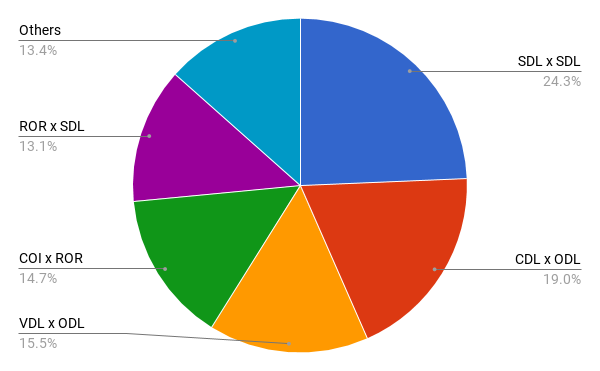
\includegraphics[scale=0.5]{images/chart-total-rules-duplicated.png}
		\caption{D-Rules that avoided more duplicated mutants.}
		\label{fig:rules-duplicated}
	\end{center}
\end{figure*}

Occurring less often, the E-Rules are applied to avoid equivalent mutants.
Figure~\ref{fig:rules-equivalents} shows that only one rule was responsible for 95.7\% of the cases found.
The problem of the AOIS (Arithmetic Operator Insertion (short-cut)) mutation operator was presented in Figure~\ref{fig:background} (Chapter~\ref{chp:introduction}).
This rule does occur very often since several methods return local variables of numeric types.

\begin{figure*}[htb]
	\begin{center}
		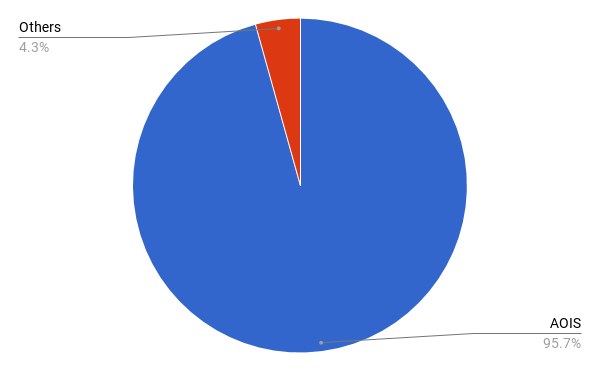
\includegraphics[scale=0.5]{images/chart-total-rules-equivalent.png}
		\caption{E-Rules that avoided more equivalents mutants.}
		\label{fig:rules-equivalents}
	\end{center}
\end{figure*}

We checked some rules that have not been confirmed by TCE, but was confirmed by the manual analysis.
In all projects TCE did not confirm any duplicated mutant generated by the AORB operator (Arithmetic Operator Replacement). 
For example, given \texttt{(x + 1)}, AORB generated mutants like \texttt{(x * 1)} and \texttt{(x / 1)}. 
Because the bytecodes are different (i.e., \texttt{imul} versus \texttt{idiv}), TCE misses these duplicated mutants. 
On the other hand, regarding the \textit{ant} project, TCE confirmed 95\%, 75\%, 60\%, and 10\% of the duplicated mutants generated by ODL x VDL, ROR x SDL, COI x ROR, and SDL x SDL.

Now we answer the research question related to the overhead of executing our rules with respect to time. 
Table~\ref{tab:execution-time} presents the execution time (in seconds) of the original \mujava{} version and the version embedded with our rules. 
For all systems, our version saved time. 
Although our rules introduce an additional overhead, the payoff amount is higher than 12\% for all projects and reached almost 20\% in two projects. 
Because we generate and compile fewer mutants, we have less I/O operations. 
These operations are more expensive than executing our rules.

\scriptsize
\begin{table}[ht]
\centering
\caption{Execution time of \mujava{} without the rules (original version) and with the rules. The presented numbers represent an average of three executions per project.}
\label{tab:execution-time}
\begin{tabular}{|l|r|r|r|}
\hline
\multicolumn{1}{|c|}{\textbf{Project}} & \multicolumn{1}{c|}{\textbf{\mujava{}  w/o Rules}} & \multicolumn{1}{c|}{\textbf{\mujava{} w/ Rules}} & \multicolumn{1}{c|}{\textbf{Difference}} \\
\hline
ant                                            & 871.57s                                                   & 745.84s                                                 & 14.43\%                                          \\ \hline
bcel                                           & 2,345.78s                                                 & 1,888.22s                                               & 19.51\%                                          \\ \hline
commons-lang                                   & 5,235.71s                                                 & 4,189.41s                                               & 19.98\%                                          \\ \hline
commons-math                                   & 430.75s                                                   & 377.3s                                                  & 12.41\%                                          \\ \hline
h2                                             & 8,097.39s                                                 & 6,680.4s                                                & 17.50\%                                          \\ \hline
joda-time                                      & 421.51s                                                   & 368.64s                                                 & 12.54\%                                          \\ \hline
\end{tabular}
\end{table}
\normalsize


\subsection{Threats to Validity}

The projects we used represents a threat to external validity. 
To alleviate this threat, we selected projects of different sizes and domains. 
Also, these projects have been used by the mutation testing community~\cite{KINTIS:2017:1, MADEYISKI:2014:1, KINTIS:2015:1}.

Our rules implementation in \mujava{} is a threat to internal validity. 
We minimize this threat because the majority of the useless mutants have been confirmed as useless by the TCE tool. 
For the remaining ones, we manually analyzed a sample of 10\% of the useless mutants identified by each rule. 
We found a few bugs in our implementation, fixed them, and re-executed the entire analysis. 
In this context, the manual analysis also represents a threat. 
We alleviate such a threat by double checking the questionable cases with a second researcher. 
Additionally, the sample represents a threat as well. 
Nevertheless, we tried to minimize this threat by sampling useless mutants identified by all rules we have implemented.

Our rules can avoid the generation of useless mutants. 
In this way, we can reduce costs not only regarding the generation itself but also on the following two tasks: compiling the useless mutants and executing the test suite against them. 
The execution time we present in Table~\ref{tab:execution-time} confirms the costs reduction. 
The calculation of the execution time also poses an internal threat since the number of I/O tasks is usually high for this type of system. 
So we tried to minimize this threat by running each project three times in each version of \mujava{} and getting the average time.

It is easy to reason about the execution time results, given that we implemented our rules by using a set of conditionals. 
So, the cost of executing a rule should not be higher than generating a mutant and compiling it. 
However, it is important to remember that we have not implemented more costly rules, e.g., the ones that need \textit{def-use} analyses. 
This is a threat to conclusion validity, given that the differences presented in the Table~\ref{tab:execution-time} can change in case we consider such rules 

%However, there is a threat to conclusion validity: these numbers do not consider rules that need \textit{def-use} analyses. 
%So, the differences presented in the table can change in case we consider such rules.


%\section{Better Discussion (RESULTS)}

%\section{Next Steps: Custo/Trade-Off, Comparing with other tools like TCE}

\section{Research Status}
In this chapter, we have demonstrated that the rules can be feasible.
Next, we list the tasks to improve this part of the research.

\begin{enumerate}
    \item \textbf{Improve the result analysis:}~We checked which rules the TCE was able to confirm in the ANT project, but we did not check the reasons that led it to confirm or not a mutant as useless. A special case we identified were the D-Rules AORB x ODL and AORB x AORB that involved the generation of different bytecodes, as explained earlier in this chapter. Further analysis of the mutants confirmed and not confirmed by the TCE will help to understand the limitations of each approach.
    \item \textbf{Implement and evaluate the rules in other mutation testing tools: }~In this work we selected \mujava{} to implement and evaluate our rules. Nevertheless, other mutation tools can also benefit from using the rules and thus avoid useless mutants. This is the case of \pit{}, where we found rules associated with its mutation operators.
    \item \textbf{Compare with other solutions:}~In the evaluation we used TCE just to validate our rules. However, it can also be used as a solution to detect equivalent and duplicated mutants. This way, after implementing a substantial number of rules in \mujava{} we can compare our technique with TCE in terms of performance to reduce the number of useless mutants and calculate the associated cost of each solution. One solution does not subsume the other, given that we can use them in combination. Besides TCE, we intend to investigate other solutions that tackle the equivalent and duplicated mutant problems and compare with our rules.
\end{enumerate}
